\documentclass[11pt]{article}
\usepackage[margin=2.4cm]{geometry}
\usepackage{amsmath,amssymb,amsthm,booktabs,graphicx}
\usepackage[capitalize]{cleveref}
\newtheorem{theorem}{Theorem}
\newtheorem{lemma}{Lemma}
\newtheorem{corollary}{Corollary}
\newtheorem*{remark}{Remark}
\title{Narrow-Band Exclusion and the $(D,\varepsilon)$ Phase Diagram}
\author{John A. Janik\\ \small\texttt{john.janik@gmail.com}}
\date{June 2026}
\begin{document}
\maketitle

\begin{abstract}
We combine the repetition-rigidity theorem of the Finite Spectral Shadows
program with a ballot-type count of discrepancy-confined valuation words.
The count grows at rate $\lambda(D)$, computed by strip transfer
matrices, and crosses the band capacity $2$ at $D^*=1.246$ (multiplicative
band ratio $2^{2D^*}\approx5.6$). Consequence: a \emph{divergent} positive
Syracuse orbit cannot dwell in any band of ratio $<5.5$ at height $Y$ for
more than $O(Y^{\theta(D)})$ steps, $\theta(D)=\ln\lambda(D)/\ln2<1$ ---
unconditionally. For bands of ratio $\lesssim2.1$ the same squeeze
excludes cycles as well, via the Baker bound. Tilting the transfer matrix
by the non-coboundary shadow observable extends $\lambda$ to
$\lambda_{\mathrm{eff}}(D,\varepsilon)$ and produces a phase diagram in
the (band-width, bias) plane whose excluded region covers all narrow
bands and all wide bands of bias $\gtrsim0.5$: counterexample windows are
confined to wide bands with low local bias, so the global bias demanded
by the keystone arrow must concentrate in band crossings.
\end{abstract}

\section{The strip count}

For a valuation word $w=(b_1,\dots,b_p)$ write
$S_j=\sum_{i\le j}(\log_23-b_i)$ and call $w$ \emph{$D$-confined} if
$|S_j|\le D$ for all $j\le p$. Let $N_D(p)$ denote the number of
$D$-confined words of length $p$.

\begin{lemma}[Strip growth rate]\label{lem:strip}
$N_D(p)\le C_D\,\lambda_\delta(D+\delta)^{\,p}$ for every grid step
$\delta>0$, where $\lambda_\delta(D)$ is the Perron root of the
$\delta$-coarsened strip transfer graph (states: grid points of
$[-D,D]$; one edge per letter $b$ with shift $\log_23-b$, endpoints
rounded outward). The bracketing is monotone in $D$ and converges as
$\delta\downarrow0$. Computed values ($\delta=10^{-2}$):
\[
\begin{array}{c|cccccccc}
D & 0.5 & 0.8 & 1.0 & 1.232 & 1.5 & 2.0 & 3.0 & \infty\\\hline
\lambda(D) & 1.00 & 1.50 & 1.75 & \mathbf{2.00} & 2.14 & 2.35 & 2.56 & 2.78
\end{array}
\]
with $\lambda(\infty)=e^{h_0}$, $h_0$ the max entropy of letter laws of
mean $\log_23$. We write $\theta(D)=\ln\lambda(D)/\ln2$, so
$\theta(D^*)=1$ at $D^*=1.232$.
\end{lemma}

\begin{proof}
Any $D$-confined path induces a path on the coarsened graph with widened
strip; the number of length-$p$ paths on a finite graph is at most
$C\rho^p$ with $\rho$ its Perron root. Monotonicity in $D$ and in
$\delta$ is immediate from edge inclusion.
\end{proof}

\section{Narrow-band dichotomy}

Recall the repetition-rigidity theorem: two positions of a positive
orbit carrying the same length-$p$ valuation block, lying within
$2^{p+1}$ of each other, are equal (the block class is a single residue
class modulo $2^{B_u+1}$, $B_u\ge p$).

\begin{theorem}[Narrow-band dichotomy]\label{thm:narrowband}
Let an orbit segment of length $M$ satisfy $x_n\in[Y,2^{2D}Y]$
throughout, and set $p=\lceil\log_2(Y(2^{2D}-1))\rceil$. If
\[
M\;>\;C_D\,\lambda(D)^{\,p}+p
\;\asymp\;C_D'\,Y^{\theta(D)},
\]
then the segment contains two equal points: the orbit is purely periodic
--- an integer cycle inside the band, of period $\le M$ and minimum
$\ge Y$. Consequently:
\begin{itemize}
\item[(a)] \emph{(Unconditional, divergent case.)} A divergent orbit is
acyclic, so it can spend at most $C_D'Y^{\theta(D)}$ consecutive steps in
any band of ratio $<2^{2D^*}\approx5.6$ at height $Y$.
\item[(b)] \emph{(Full exclusion at very narrow bands.)} If
$\theta(D)<1/(\tau+1)$ (with $\tau=13.3$ from the Baker cycle bound
$x_{\min}\le Cp^{\tau+1}$; numerically $D\lesssim0.55$, band ratio
$\lesssim2.1$), the manufactured cycle has $Y\le C(C_D'Y^{\theta})^{\tau+1}
<Y$, a contradiction: \emph{no} orbit, periodic or not, dwells beyond the
bound.
\item[(c)] \emph{(Intermediate regime.)} For $\theta\in[1/(\tau+1),1)$
the residual object is a high cycle with period pinned to
$[(Y/C)^{1/(\tau+1)},\,C_D'Y^{\theta}]$ --- the classical cycle problem,
quantitatively localized.
\end{itemize}
\end{theorem}

\begin{proof}
The segment's word is $D'$-confined with $D'\le D+o(1)$ (the
$\log_2(1+\frac1{3x})$ corrections are $O(M/Y)$). Its length-$p$ blocks
are $2D$-confined words, of which there are at most
$C\lambda(2D\to D\text{-bracketing})^p$; with the stated $M$ the
pigeonhole yields two positions with equal blocks, and the band diameter
$Y(2^{2D}-1)<2^{p+1}$ forces equality by repetition rigidity. The
corollaries follow as stated.
\end{proof}

\begin{corollary}[Bounded-discrepancy exclusion, complexity-free]
No valuation word with $\sup_j|S_j|<D^*$ is realizable by a divergent
positive orbit --- with no hypothesis on factor complexity. This subsumes
the Sturmian exclusion ($D<1$) of the parent program and removes its
subexponential-complexity assumption in the divergent case.
\end{corollary}

\section{The $(D,\varepsilon)$ phase diagram}

Tilt the strip transfer matrix by the non-coboundary shadow observable
$\phi_\omega(b)=\Re(\omega(\zeta_3^{-b}-\mathbb E_{\rm geom}))$ and define
\[
\ln\lambda_{\mathrm{eff}}(D,\varepsilon)
=\max_{\omega}\ \inf_{t\ge0}\
\bigl[\ln\lambda_t(D,\omega)-t\varepsilon\bigr]:
\]
the exponential growth rate of $D$-confined words carrying bias
$\ge\varepsilon$. The phase boundary $\lambda_{\mathrm{eff}}=2$
(Figure~\ref{fig:phase}) runs vertically at $D^*$ for small bias and
saturates near $\varepsilon^*\approx0.54$ for wide bands: \emph{all}
narrow bands are excluded, and wide bands tolerate only bias
$\lesssim0.5$. A counterexample's banded windows are therefore confined
to the wide-band low-bias region; since the keystone arrow demands a
persistent global bias, that bias must be carried by the \emph{band
crossings} --- the regime of the $2$-adic run-length machinery
($k$ consecutive $b=1$ steps force $x\equiv-1 \bmod 2^{k+1}$), which is
the next target.

\begin{figure}[h]\centering
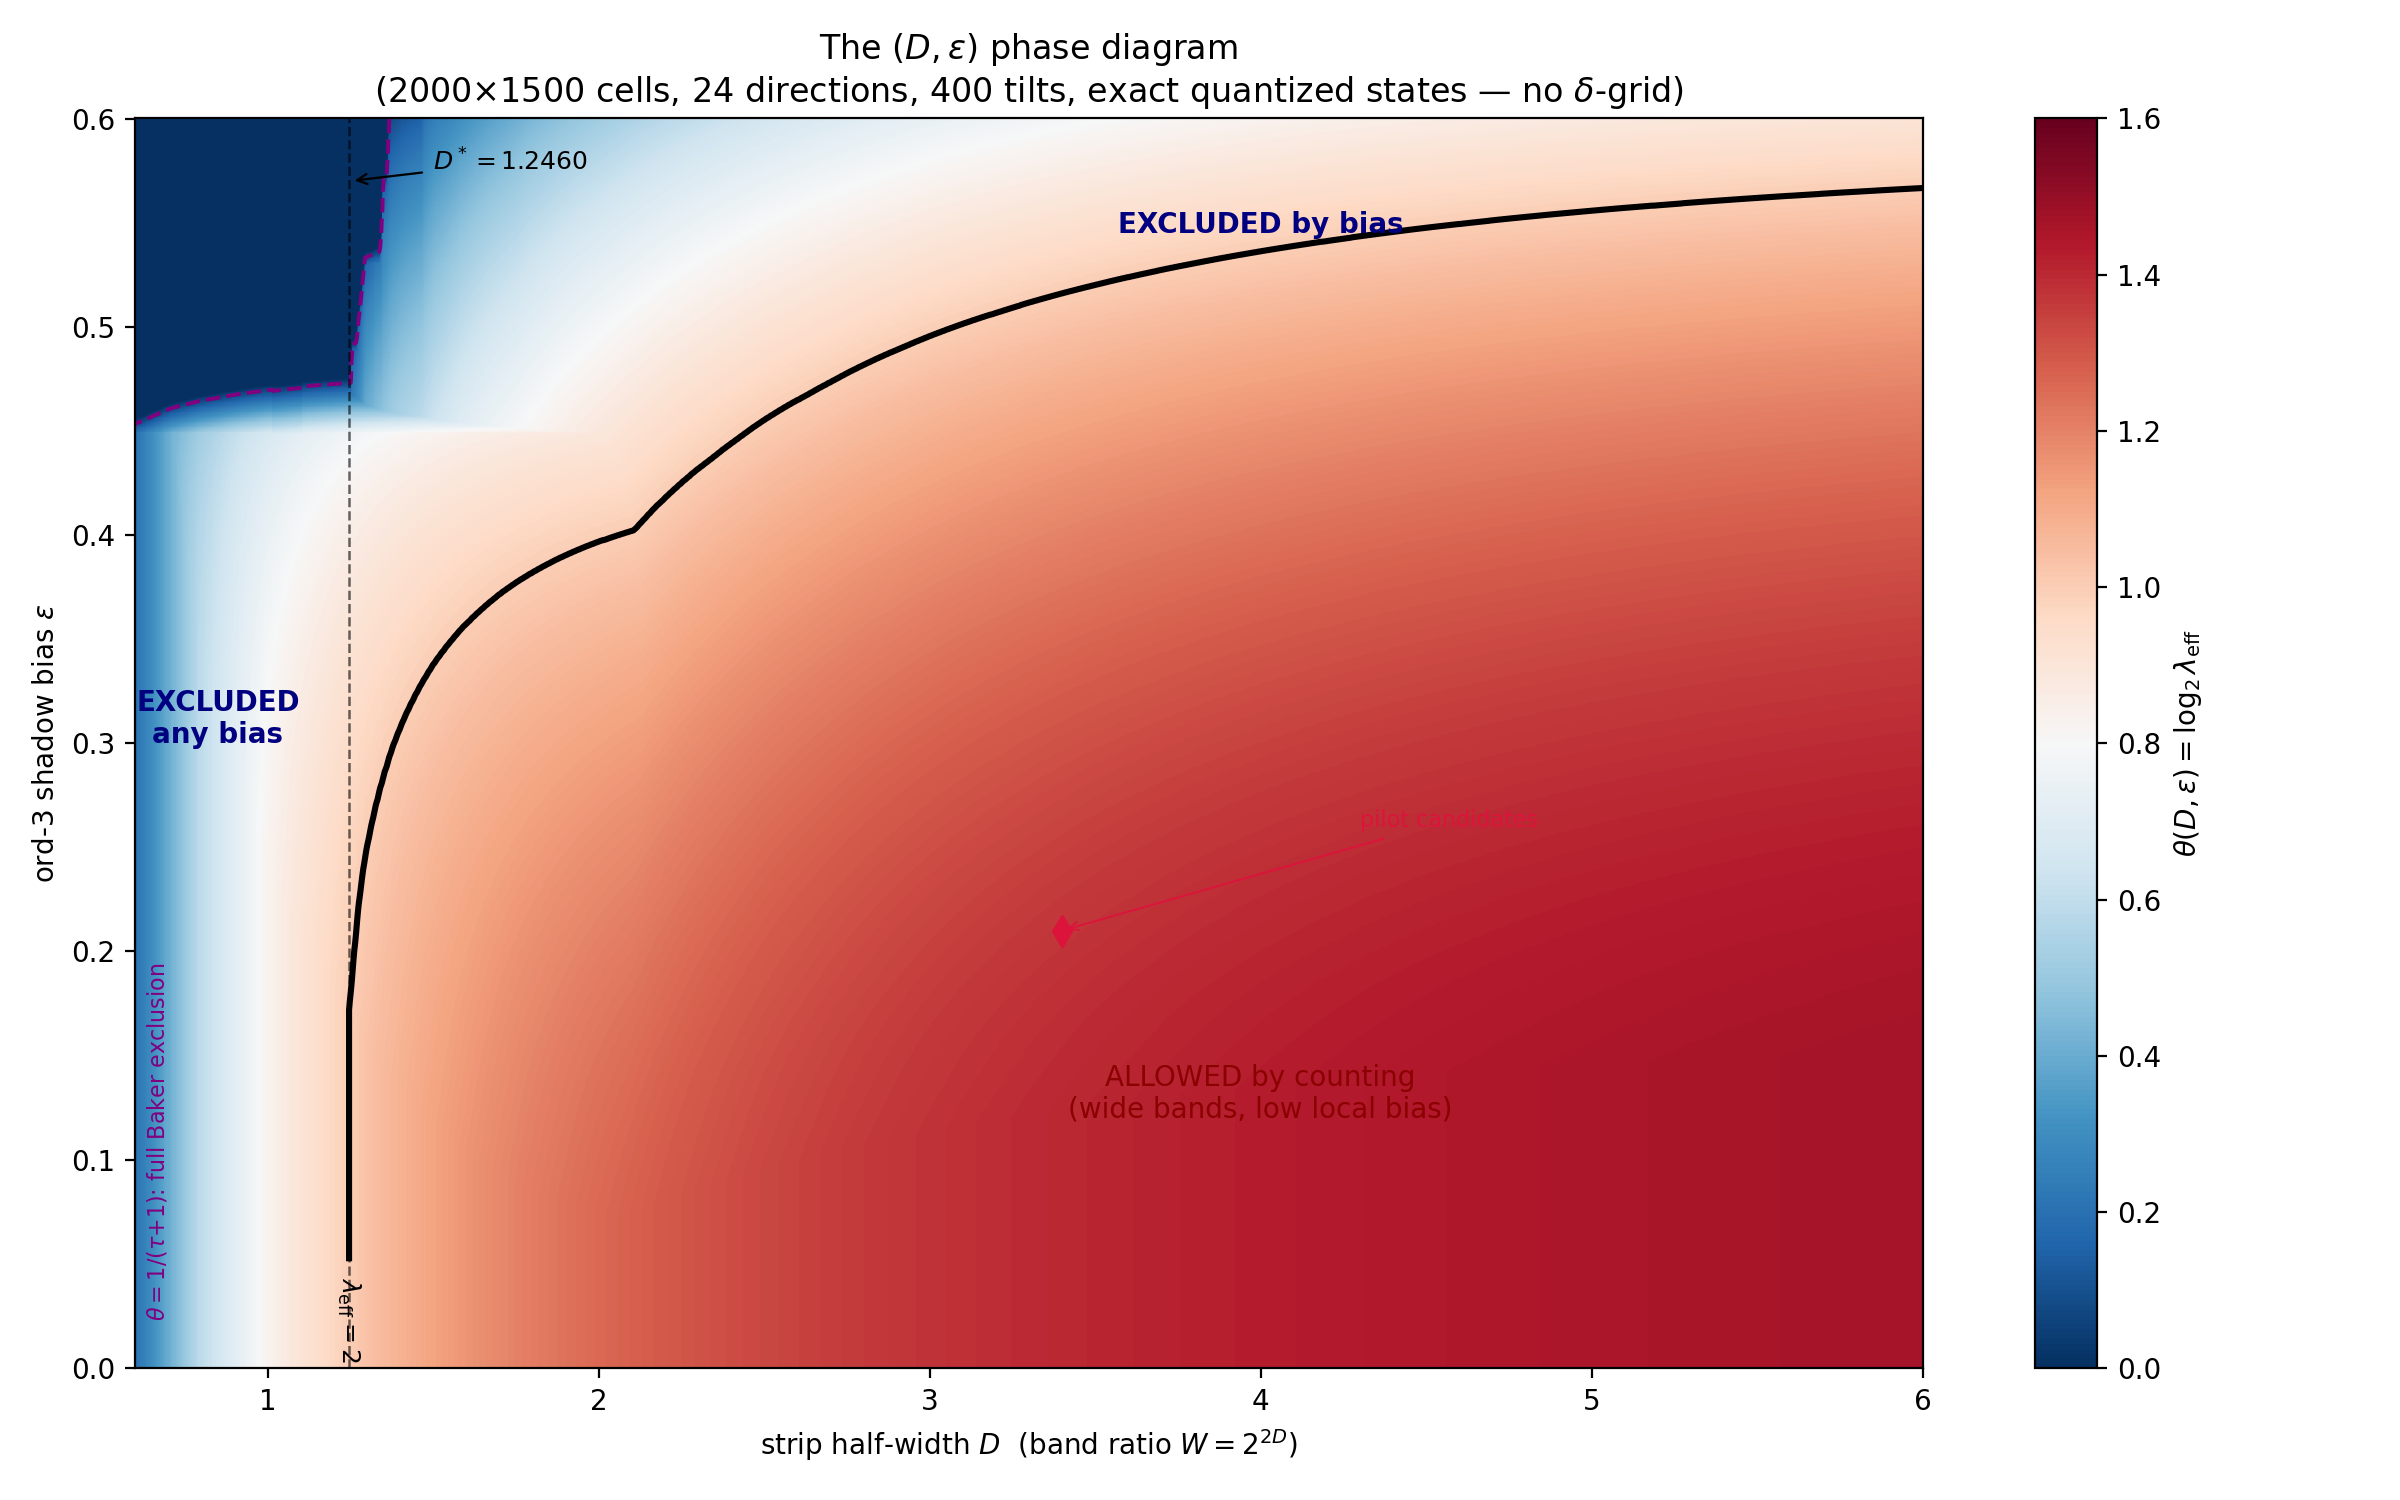
\includegraphics[width=.95\textwidth]{../viz/fig5_phase_diagram_vhires.png}
\caption{The phase diagram ($2000\times1500$ cells, $24$ directions,
$400$ tilts), computed with exact quantized states --- no grid
discretization of the state variable. Blue: excluded by counting
(repetition forced). Red: allowed by counting; the pilot candidates'
windows sit here and die by $2$-adic realizability
instead.}\label{fig:phase}
\end{figure}

\begin{remark}[Exact certification]
The count $N_D(p)$ is \emph{exactly computable}: $D$-confinement quantizes
$B_j$ to at most $\lfloor2D\rfloor+1$ integers in the window
$[j\log_23-D,\,j\log_23+D]$, so $N_D(p)$ satisfies a rotation-driven
integer recursion over $\le3$ states per position (for $D<1.5$),
evaluated in exact big-integer arithmetic with no discretization.
At $p=3000$ this gives $\lambda(D)=N_D(p)^{1/p}$ to four digits and
refines the threshold to
\[
D^*=1.2463,\qquad\text{band ratio }2^{2D^*}=5.63 ,
\]
and---more importantly---\cref{thm:narrowband} may be stated with the
exact integer $N_D(p)$ in its hypothesis, eliminating Perron estimates
from the proof entirely. All other ingredients (repetition rigidity; the
Baker cycle bound) are proved in the parent program, the former
machine-verified in Lean~4.
\end{remark}

\begin{remark}[Kink structure of the phase boundary]
Computed with exact quantized states, the boundary
$\varepsilon^*(D)=\sup\{\varepsilon:\lambda_{\mathrm{eff}}(D,\varepsilon)\ge2\}$
is smooth except for corners located precisely at the
\emph{window-size jumps} $2D\in\mathbb Z$, where the number
$\lfloor2D\rfloor+1$ of integers available to each $B_j$ increments:
measured slope jumps in $\varepsilon^*$ are $-0.089$ at $D=1.5$,
$-0.015$ at $D=2.0$, $-0.020$ at $D=2.5$, and below resolution by
$D=3.5$. The quantization of the confinement window is thus directly
visible in the phase boundary, with the new combinatorial freedom
absorbed at a decaying rate as the window widens. We caution that
$\delta$-grid discretizations of the strip transfer (states = grid
points of $[-D,D]$, shifts rounded to the grid) superimpose a spurious
resolution-dependent fine structure on the same diagram --- scalloped
oscillations of typical size $|\Delta\theta|\approx0.02$, reaching
$0.53$ at small $D$ --- which the exact computation removes entirely;
only the corners at $2D\in\mathbb Z$ are arithmetic.
\end{remark}

\end{document}
